\chapter{Discussion}
In this chapter we are discussing what conclusions we can draw from our results presented in sec. \ref{sec:results} and in which directions future research could go.

% =======================================
\section{Conclusion}
% =======================================
\subsection{The Quality of Our Topic Models}
The results from our measurements regarding the quality of our topic models indicate that the created topic models tend to be stable in their quality when varying the seed and even with slightly changed dictionaries. Furthermore, topic models created with classic LDA tend to have a higher quality than the ones created with neural LDA. Topic models from neural LDA have an interesting inverse peak at 3 topics and tend to produce topic models with nearly the same quality for a topic size of 5 or more when using ancestral sampling.

In the original papers of GPT-2 \cite{gpt-2} and Transformer-XL  \cite{transformer-xl}, the coherence score $C_v$ for their testset is between $0.35$ and $0.60$. Thus, our topic models have a good correlation to human topic-ranking data, especially those with a higher number of topics which can be seen in table \ref{fig:summary}. Regarding different sampling techniques, we see that on average Top-P and even more so Typical sampling clearly improve the quality of topics created by topic models.  
\begin{figure}[H]
    \centering
    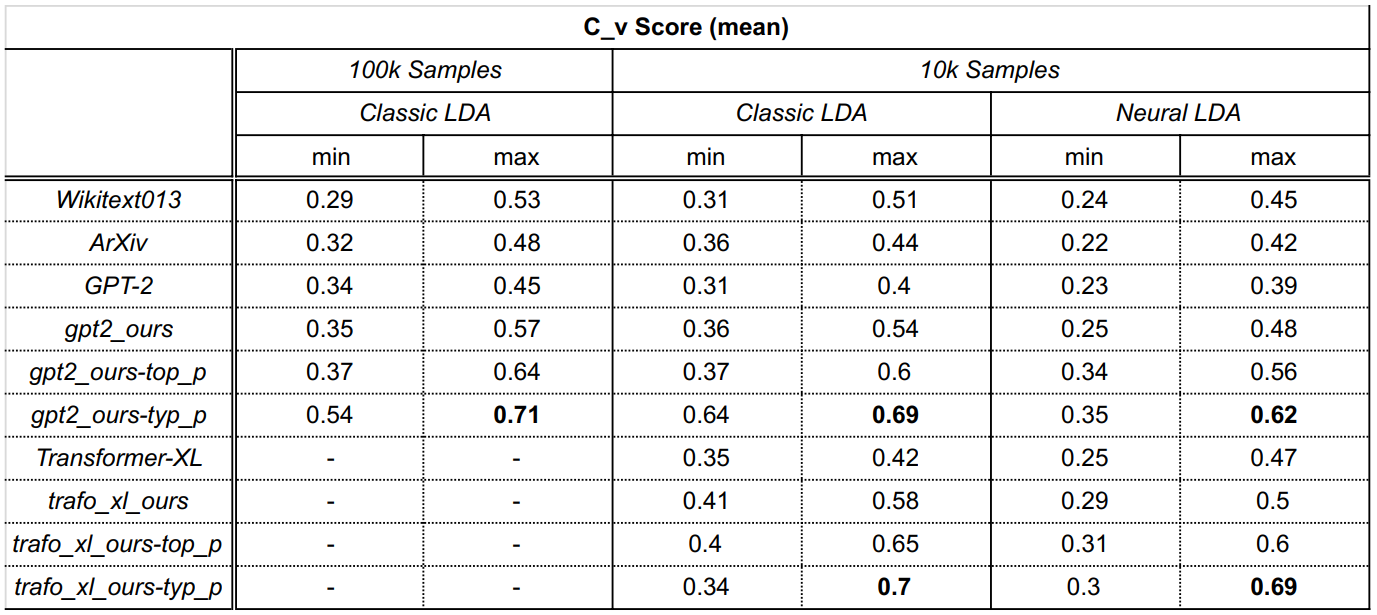
\includegraphics[width=1\textwidth]{figures/Unigrams-cv-var-table-is}
    \caption{$C_v$ topic coherence score table with min and max mean values computed over all topic models.}
\label{fig:summary}
\end{figure}

% =======================================
\subsection{Comparing the Semantic Spaces}
The results from the comparison between topic models with corpora of 100'000 documents clearly show dissimilarities between the sampled corpus and the corpus the GPT-2 model was trained on. With our variance analysis, we can say with a good degree of confidence that these findings are solid for a topic size of 10 or more. In general, we expect the two topic distributions from training dataset and generated dataset to be similar, as the goal of our language model is to learn the language of the corpus it is trained on. This indicates that there is something that skews the model's topic distribution. To find out what is causing this, we have to look at the results from the comparison of topic models with corpora of 10'000 documents. 

First, through our variance analysis for topic models of corpora with 10'000 documents, we have to take a variation of up to $0.1$ for a topic size of 5 or more into account. This makes the interpretation rather vague and we conclude that topic models from corpora with 10'000 documents are not ideal for interpretations. Nonetheless, in our comparison we see that dissimilar topic models result in a value of $0.5$ or higher. This strongly correlates to our findings with corpora of 100'000 documents. For similar topic models, the values tend to be under $0.2$ for a topic size of 10 or lower. For a topic size higher than 10, the area of similar topic models tends to be under $0.4$. This differs from our first findings where the area for similar topic models remains under $0.2$ across all topic sizes. The comparison of the topic models from the sampled corpus and the corpus the GPT-2 model, respectively the Transformer-XL model, was trained on, lies in the area of similarity. This again differs from our first findings where we see a clear discrepancy. We can conclude that if there is a strong inductive bias from the model architecture, we can assume we would see some discrepancies even in topic models from corpora with just 10'000 documents. 

Concerning the differences between the GPT-2 and Transformer-XL results, we expect the topic models created from the original Transformer-XL model to behave similarly to the model we trained ourselves. This is because the original Transformer-XL model was also trained on the Wikitext103 corpus. This assumption is reflected in our results for \texttt{trafo\_xl\_ours} vs. \texttt{trafo\_xl}. It also makes sense that the results from GPT-2 and Transformer-XL did not differ much. Both underlying architectures are based on the decoder model from the Transformer architecture. It backs our proposed approach because we can see similar results with a similar language model architecture. 

As for the differences between the classic LDA and the neural LDA, we come to the same conclusions as with classic LDA. The difference of the learned semantic space and the original one tend to appear similar. There is no clear indication that something skews with the topic distributions. What can clearly be seen in the graphs is that both topic model techniques have the same area of similarity and area of dissimilarity for a corpus size of 10'000 documents. This also backs our proposed approach as the produced results are very similar across different topic modeling techniques.

As for corpora created with different sampling techniques (ancestral, Top-P and Typical sampling), we see that different sampling methods always lead to a skewed topic distribution. By looking at the red lines in all the graphs with all three sampling methods (sec. \ref{sec:comp}, the graphs on the right), we can see that Top-P sampling and even more Typical sampling in general influence the topic distributions. We therefore conclude that the sampling methods Top-P and even more so Typical sampling introduce a generalization to the predicted output which overrules some of the meanings in the semantic spaces. Such an impact is rather unlikely if there is a strong inductive bias in the language model architecture.

% =======================================
\subsection{Summary}
With our new approach to probing language models, we show that by analyzing the differences from various topic distributions, we gain a better understanding of the characteristics of the language learned by today's language models. Furthermore, we are closer than before to being able to identify the isolated impact the inductive bias has on our metric. With this, we show a way to finding out what components of the learning algorithm lead to certain inductive biases. We find discrepancies in the semantic space that are linked to the different methods and parameters we applied but also to the language model algorithm itself. We give a baseline for how to use our method, and build a foundation on which further research can be built. 

% =======================================
\section{Further Work}
After providing the groundwork, our method can be further enhanced and explored in various ways. 

By focusing on the topic model part, the method itself can be extended to work with non-LDA-based topic models \cite{karami2018fuzzy, zhang2022pre}. Additionally, a different approach to tokenization and dictionary creation can lead to more stable and more meaningful topic models which is reflected in the metric. This can help to better identify the differences in the semantic space over corpora of different sizes. We tried incorporating bigrams and trigrams into our topic models but could not to see any notable difference between them. This does not mean they have no influence, just that our implementation did not show any.

By putting the focus on the language model, the method itself can be extended to work with other language model architectures, e.g. encoder based architectures. Additionally, different approaches to train the language model, like changing the loss function and the training parameters, can provide an insight into the influence of architectural properties on the semantic space. All in all, comparing the behaviour of our metric with different language models might tell us what components of the learning algorithm lead to certain inductive biases, which leads in itself to a change in the choice of language model for specific downstream tasks.

Furthermore, by changing the training data for the language models, i.e. using a completely different dataset or an altered version, can give us an insight into how the inductive bias of one language model architecture affects the learning behaviour with different learning data. This might lead to conclusions on how today's language models are trained and how we utilize training data. 

We also suggest to test the stability of our method for a higher corpus size than 10'000 documents, as this will provide answers to how reproducible the results of our metric are and how the language models inductive bias is reflected on different corpus sizes.

If we consider a totally different direction instead of focusing on the inductive bias, we can shift our view to how we can utilize the learned topic distributions from a language model. We could try to influence the probability of a produced string of a language model by combining the learned topic distribution with the intermediate conditional probability over words from a language model. This could help us increase the probability of a string with a certain topic, which is especially interesting when the topic is not very common in the learned language. By analyzing the topics themselves, we could see where the semantic space differs on a word level. Comparing the topic-word distributions with the results or findings from downstream tasks, we could draw conclusions about what specific bias those models exert in those downstream tasks. 